\documentclass{article}

\usepackage[a4paper, top=1cm, bottom=2cm, left=2.5cm, right=2.5cm]{geometry}
\usepackage{graphicx}
\usepackage{hyperref}
\usepackage{authblk}


\title{\textbf{Traduction vidéo de langage des signes en texte}}
\author{
    Bertrand Awenze$^{1}$, Christian Nebot$^{2}$, John-William Lebel$^{3}$, Gabriel Anjuère$^{4}$, Lucas Ambinintsoa$^{5}$
}

% Affiliations en une seule ligne avec exposants
\affil[ ]{$^{1,3}$ GLO-4030 \quad $^{2,4,5}$ GLO-7030}


\date{\today}

\begin{document}

\maketitle

\noindent
\textbf{Objectif} \\

L’objectif de ce projet est de créer et d’entraîner un modèle capable de traduire une vidéo en langage des signes en texte.\\ 

\begin{figure}[h]
    \centering
    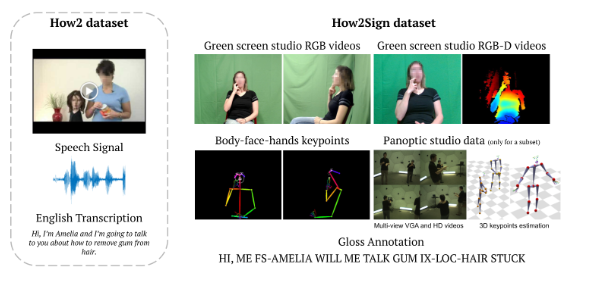
\includegraphics[width=1\textwidth]{img/image.png}
    \caption{Présentation du projet}
\end{figure}

\noindent
\textbf{Pourquoi avoir choisi ce projet pour GLO-7030 ?} \\
\begin{itemize}
    \item Peu de modèles existants pour cette tâche.
    \item Disponibilité d’un nouveau jeu de données de haute qualité.
    \item Possibilité d’explorer plusieurs approches et architectures.
\end{itemize}

\noindent
\textbf{Proposition de méthodologie} \\

Notre approche consiste à combiner différentes architectures, notamment des autoencodeurs et des transformers, afin d’effectuer la conversion des images et du son en texte. \\

Dans un premier temps, un prétraitement des données sera nécessaire. La grande dimensionnalité des données, due à leur haute qualité, nécessite une réduction. Nous envisageons de réduire la résolution des vidéos afin d’améliorer la généralisation des modèles. 
De plus, le fond vert présent dans le jeu de données pourra être changé pour augmenter les données. \\

Nous débuterons l’entraînement sur un sous-ensemble du jeu de données, ce qui nous permettra d'évaluer les architectures avant de passer à l’ensemble des données. 
Une fois la bonne architecture choisie, nous procéderons à l’entraînement sur l’intégralité du jeu de données.\\

Les données nécessaires à cette tâche sont accessibles via le site suivant :  
\href{https://how2sign.github.io/}{How2Sign}

\end{document}
